\documentclass[a4paper, 12pt]{article}
\usepackage[utf8]{inputenc}
\pagestyle{empty}
\usepackage[usenames]{color} %used for font color
\usepackage[russian]{babel}
\usepackage{amssymb} %maths
\usepackage{amsmath} %maths
\usepackage{wrapfig}
\usepackage{xcolor}

\usepackage{chapterbib}

\usepackage{natbib}
\usepackage{graphicx}
\usepackage{hyperref}
\usepackage{bigints}

\usepackage[normalem]{ulem}  % для зачекивания текста

\definecolor{linkcolor}{HTML}{0000FF} % цвет ссылок
\definecolor{urlcolor}{HTML}{0000FF} % цвет гиперссылок
\hypersetup{pdfstartview=FitH,  linkcolor=linkcolor,urlcolor=urlcolor, colorlinks=true}

\oddsidemargin = 0 pt
\textwidth = 18 cm
\marginparsep = 0 pt
\marginparwidth = 0 pt
\hoffset = -0.41 in

\headheight = 0 pt
\headsep = 0 pt
\topmargin = 0 pt
\voffset = -0.4 in
\textheight = 10.511 in

\graphicspath{{pictures/}}
\DeclareGraphicsExtensions{.pdf,.png,.jpg}

\begin{document}
   \begin{center}
  \textbf{1-ое занятие по алгоритмам.} 
 \end{center}

 \textbf{Поток(flow).} Это математический объект. Мы можем рассматривать как водопроводную сеть, которая представлена в виде взвешенного ориентированного графа. В графе есть две(может больше) особенные вершины - исток и сток. Мы хотим "перегонять" как можно больше воды в секунду.

 \textbf{Сеть} - это ориентированный граф. $c: E \to \mathbb{R} $ - пропускная способность, $e \in V$ - исток,\break$t \in V$ - сток.

  \textbf{Поток} - это функция $f: E \to \mathbb{R} $ которая возвращает поток по ребру. В котором выполняется два правила. (1) Сумма входящей воды равна выходящей. (2) По ребру проходит воды не больше чем его пропускная способность.

  \textbf{Величина потока.} $|f|_t = $ сумма входящих в сток минус сумма всех исходящих из стока.  $|f|_s = $ сумма выходящих из истока минус сумма всех входящих из истока. На самом деле эти суммы равны, доказательство заключается в том что в каждую вершину входит столько же воды сколько и выходит, но в исток "свыше" приходит вода, значит она куда-то должна деться, очевидно что только в сток.

\textbf{Доказательство существования максимального потока.} У потоков есть точная верхняя грань, возьмем последовательность потоков подходящей к точной верхней грани. Выберем какое-то ребро и возьмем бесконечную сходящуюся подпоследовательность из нашей последовательности для ребра. Проделаем данную операцию для каждого ребра, возьмем предел для каждого ребра, все свойства будут выполняться.

Просто искать пути и заполнять их - нельзя. Есть пример даже без циклов, если мы выбрали путь, который блокирует другие пути.

\begin{center}
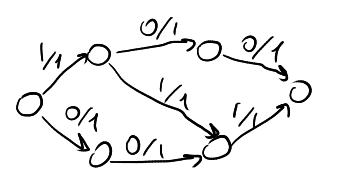
\includegraphics{img1.png}
\end{center}

\textbf{Опр.} Пусть есть сеть и поток, тогда остаточной сетью назовем сеть в которой пропускную способность заменим на (пропускную способность минус поток) и добавим обратное ребро с весом потока.

\textbf{Утв.} Если в остаточной сети есть путь по не нулевым ребрам, то поток не максимален.

  \begin{center}
 \textbf{2-е занятие по алгоритмам 09-04}
\end{center}

  \textbf{Другое определение потока.} Сеть - это $\langle V, c, s, t \rangle$, где c - это таблица смежности для всех пар вершин(таблица не симметричная).  \textbf{Поток} - это $f : V \times V \to \mathbb{R} $, такая что\break $(1) \forall u, v \in V: f(u, v) \leqslant c(u, v), (2) \forall u, v \in V: f(u, v) = - f(v, u), (3) \forall v \in V \setminus \{s, t\}: \sum\limits_{u\in V}^{}f(u, v)=0 $

  \textbf{Все следующие действия производятся с данным определением потока.} 

  \textbf{Величина потока и доказательство равенства двух определений.} $|f|_s = \sum\limits_{u\in V}^{} f(s, u), |f|_t=\sum\limits_{u\in V}^{} f(u, t)$. $0 = \sum\limits_{u, v \in V}^{} f(u, v) = \sum\limits_{u\in V}^{} f(s, u) - \sum\limits_{u\in V}^{} f(u, t) = |f|_s - |f|_t$.

  \textbf{Разрез.} Пусть есть сеть, тогда разрез - это два множества $(S, T): S \sqcup T = V, s \in S, t \in T$

   \textbf{Чистый поток через разрез.} Пусть есть сеть и разрез, тогда чистый поток через разрез - это $f(S, T) := \sum\limits_{u\in S, v\in T}^{}f(u, v) $

   \textbf{Пропускная способность разреза} - это $c(S, T) = \sum\limits_{u\in S, v \in T}^{} c(u, v)$

   \textbf{Утв.} $f(S, T) \leqslant c(s, T)$

   \textbf{Лемма.}  $\forall (S, T): f(S, T) = |f|$. Доказательство: $|f| = \sum\limits_{u\in S}^{} \sum\limits_{v \in V}^{} f(u, v) + \sum\limits_{u \in T}^{} \sum\limits_{v\in V}^{} f(u, v) =\break= \sum\limits_{u\in S}^{} \sum\limits_{v \in T}^{} f(u, v) = f(S, T)$

   \textbf{Следствие.} $\forall (S, T) |f| \leqslant c(S, T)$

    \textbf{Остаточная сеть} - это $c(u, v) = c(u, v) - f(u, v)$

     \textbf{Теорема.(Форда-Фалкерсона).} Пусть есть сеть, тогда следующие утверждения эквивалентны.
  \begin{enumerate}
    \item f - максимальный поток
    \item В остаточной сети нет пути по не насыщенным ребрам.
    \item $|f|=c(S, T)$ для какого-то разреза.
  \end{enumerate}
  $1\Rightarrow 2$ очевидно. $3 \Rightarrow 1$ очевидно. Доказательство $2 \Rightarrow 3$, например, можно удалить все насыщенные ребра, получится хотя бы две компоненты, очевидным способом выберем разрез.

  \textit{*** Тут гуляют примеры задач, но зачем их записывать? ***}

  Метод \textbf{Форда-Фаркенсона} пока можем находим путь из $s$ в $t$ по ненасыщенным ребрам и пускаем по нему сколько можем. Этот алгоритм верен для целых чисел, но если числа не целые, то алгоритм может \href{https://ru.wikipedia.org/wiki/%D0%90%D0%BB%D0%B3%D0%BE%D1%80%D0%B8%D1%82%D0%BC_%D0%A4%D0%BE%D1%80%D0%B4%D0%B0_%E2%80%94_%D0%A4%D0%B0%D0%BB%D0%BA%D0%B5%D1%80%D1%81%D0%BE%D0%BD%D0%B0#%D0%9F%D1%80%D0%B8%D0%BC%D0%B5%D1%80_%D0%BD%D0%B5_%D1%81%D1%85%D0%BE%D0%B4%D1%8F%D1%89%D0%B5%D0%B3%D0%BE%D1%81%D1%8F_%D0%B0%D0%BB%D0%B3%D0%BE%D1%80%D0%B8%D1%82%D0%BC%D0%B0}{не завершиться}.
  Асимптотика будет $O(|f|(V+E)), O(kE), O(VE)$. Выбирай любую.

  \textbf{Утв.} Пусть в сети ищется поток ФФ, пусть в какой-то момент времени от вершины $v$ до вершины $t$ нет пути, тогда после этого момента такой путь от $v$ до $t$ не появится никогда. Доказательство на пальцах. 

  \textit{*** Тут гуляют примеры задач, но зачем их записывать? ***}

  \begin{center}
  \textbf{3-е занятие по алгоритмам.} 
\end{center}
  Алгоритм \textbf{Эдмондса-Карпа} - это метод ФФ, но с поиском пути BFS.

  \textbf{Утв.} Расстояние(по количеству ребер) от произвольной $s$ до произвольной вершины $v$ в процессе алгоритма не уменьшается. \textbf{Доказательство.} Пусть мы ищем произвольный путь.

  \begin{center}
    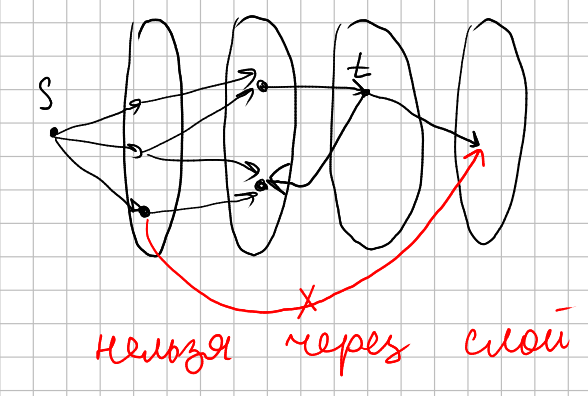
\includegraphics[scale=0.5]{img2.png}
  \end{center}
  
  Заметим, что если мы пустим поток через путь, то вершина не перескочит в слой левее, значит утверждение верно.

  Рассмотрим сколько раз могло насытиться ребро. Заметим, что если ребро насытилось несколько раз, то между этими насыщениями ребро когда-то разнасытилось, тогда рассмотрим в каких слоях находятся эти вершины.

  \begin{center}
    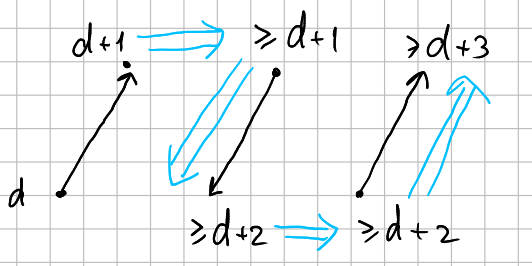
\includegraphics[scale=0.5]{img3.png}
  \end{center}

  Значит насыщений ребра могло быть только $\cfrac{V}{2}$. Ребер всего $2E$. Значит алгоритм работает за $\operatorname{O} (VE^2)$

  Давайте заметим, что если расстояние от $s$ до $t$ не увеличивается, то нам не надо перезапускать BFS.

  \textbf{Концепция блокирующих потоков} - пока у нас есть ненасыщенный путь мы находим слоистую сеть и находим блокирующий поток в слоистой сети.

  \textbf{Слоистая сеть} - это первая картинка, но мы временно игнорируем обратные ребра и внутри слоя. 

  \textbf{Блокирующий поток} - это такой поток, что мы не можем найти путь, который не содержит обратных ребер.

  Наша концепция завершится, потому что каждая итерация нашего цикла увеличивает расстояние между вершинами от $s$ до $t$, строго увеличится.

  Рассмотрим алгоритм поиска блокирующего потока. Если ребро насытилось, то мы про него забываем, если мы прошли по ребру и дальше не нашли путь до $t$, то тоже про ребро забываем. Заметим, что теперь DFS по слоистой сети работает за $V + E_{\text{удаленные}}$. Значит поиск блокирующего потока происходит за  $VE$. Чтобы забывать ребра можно как-то пронумеровать ребра исходящие из каждой вершины и еще хранить число сколько ребер мы забыли. Итоговый алгоритм работает за $O(V^2E)$

  \newpage
  \begin{center}
    \textbf{Целочисленные сети.}
  \end{center}

  \textbf{ Единичные сети.} Давайте посмотрим на алгоритм Диницы, заметим, что мы удаляем все ребра по которым прошли, значит поиск блокирующего будет за $E$. Давайте заметим, что всего итераций поиска блокирующего потока будет не больше чем $2 \sqrt{E}$. \textbf{ Доказательство } Рассмотрим сеть после $\sqrt{E}$ поиска блокирующего потока, продолжим алгоритм и посмотрим на поток, заметим что все пути больше $\sqrt{E}$, значит фаз будет не больше $\cfrac{E}{\sqrt{E}}$. Значит в итоге Диница работает за $\operatorname{O} (V \sqrt{E})$.

\end{document}
